
\section{Results}


\subsection{CC efficiency}




The absolute efficiency is crucial for the Compton camera performances. It affects directly the number of detected events by the camera and so the reconstruction quality of those events.
The absolute efficiency $\epsilon$ is defined as :
\begin{equation}
\epsilon =\frac{N\gamma_{recons}}{N\gamma_{total}},
\end{equation}
\label{eq:equation_efficacite_absolue}
with $N\gamma_{recons}$ the number of gamma events in coincidences,\newline
\hspace*{1cm}$N\gamma_{total}$the total number of gamma emitted: $10^8$.\newline

The absolute efficiency is presented in function of the localization of a monoenegertic gamma point source in comparison to the Compton camera center. The setup is the same as figure \ref{fig:fig_setup_CC_simulation_Hadronth}, but the point source is in the air and not in a PMMA phantom.
The point source is moved from $- 300$ mm to $+300$ mm with a step of 20 mm following the transverse axis of the camera (axis $y$) and the gamma source is monoenergetic [300 keV, 6 MeV]. \newline
The figure \ref{fig:fig_Efficiency_CC_simulation_Hadronth} shows the absolute Compton camera efficiency in function of the gamma source position. The figure \ref{fig:fig_Efficiency_CC_simulation_Hadronth_NoCuEnergy} gives the results without any cut in energy on the detectors and the figure \ref{fig:fig_Efficiency_CC_simulation_Hadronth_cutEnergy} is with a cut applied on the energy deposited in the detectors:  50 keV for the scatterer and 100 keV for the absorber.

\begin{figure} [!hbtp]	
\centering
\caption{Absolute Compton camera efficiency function of the gamma source position. The figure \ref{fig:fig_Efficiency_CC_simulation_Hadronth_NoCuEnergy} shows the camera efficiency with no energy cut applied. It models the perfect Compton camera. The figure \ref{fig:fig_Efficiency_CC_simulation_Hadronth_cutEnergy} takes into account cuts in energy: 
50 keV for the scatterer and 100 keV for the absorber. The value of the energy cut can be different for the final prototype depending of the detector energy resolutions reach. The analysis is done for energies from 300 keV to 6 MeV.}
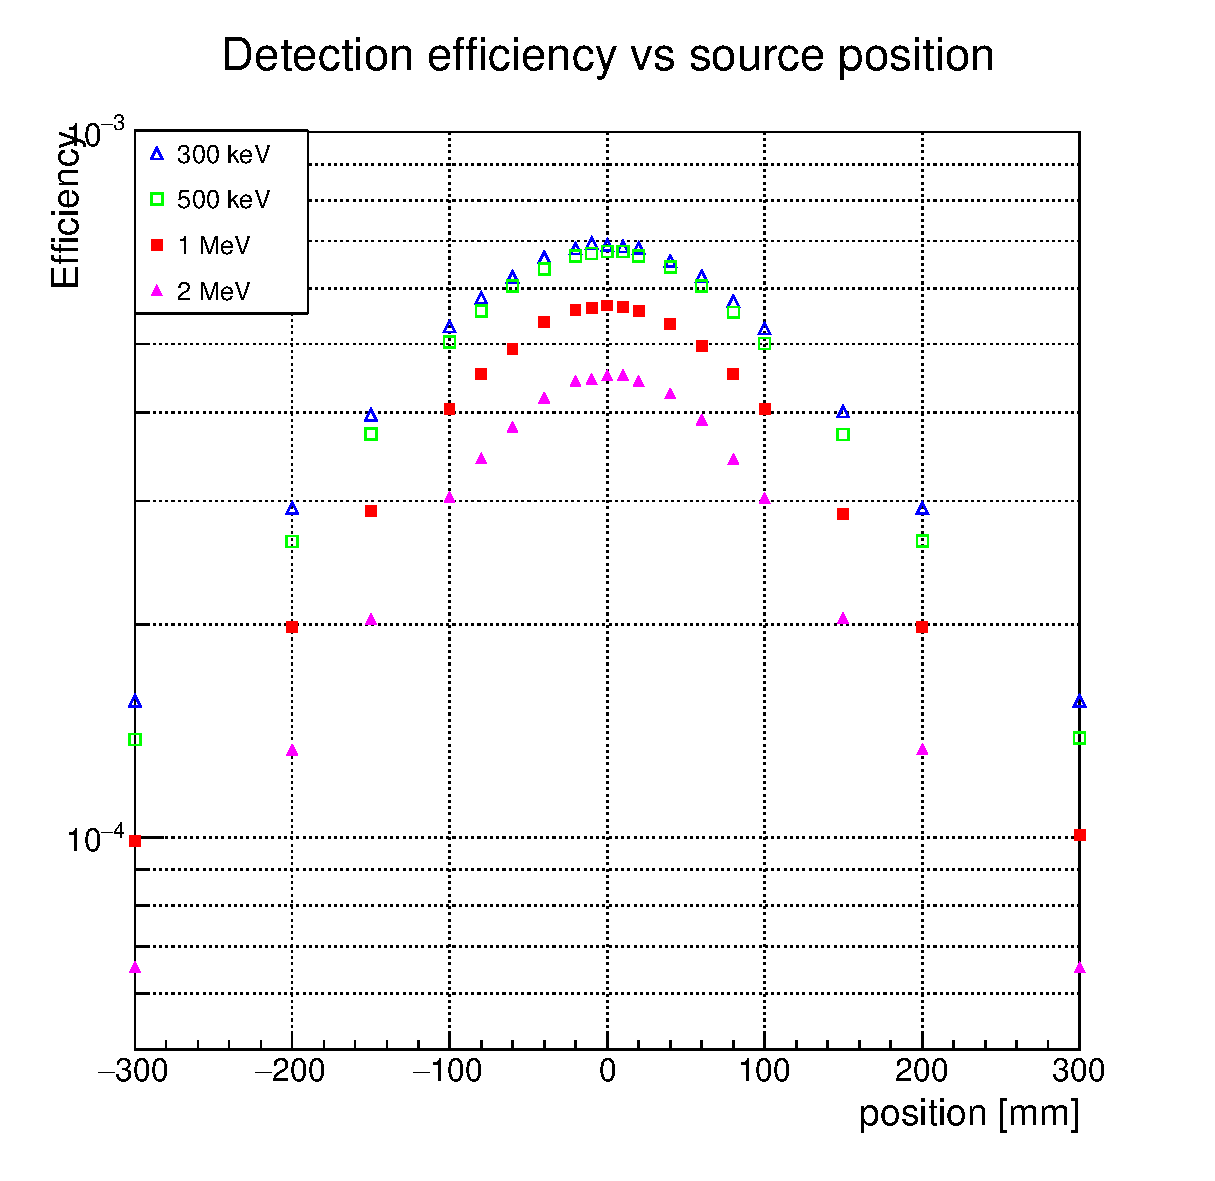
\includegraphics[width=0.7\textwidth]{./Figure/2017-06-26_Efficiency_CC_articles.eps}
\end{figure}

The absolute efficiency is between $4\times10^{-4}$ at 300 keV and $1.5\times10^{-4}$ at 6 MeV (figure \ref{fig:fig_Efficiency_CC_simulation_Hadronth_NoCuEnergy}). The efficiency is higher for low gamma energies because the probability of interaction in the absorber is decreasing with the energy. Moreover, when the point source is far from the camera center, the efficiency drops quickly. This effect is marked for high energies. In fact, the incident gamma will be less deflected in the scatterer for the same energy deposited compared to a low energy gamma. The incident gamma of interest in hadrontherapy are around 1 MeV, so it is important to well positioned the Compton camera to optimise the efficiency.\newline
Another aspect to taking into account is the energy cut applied to the detectors (figure \ref{fig:fig_Efficiency_CC_simulation_Hadronth_cutEnergy}). The detectors are not perfect and cuts are mandatory to eliminate the electronic noise. If a gamma has a small Compton scattering angle, the energy deposited in the scatterer will be small. That is why, the camera efficiency decreases when the gamma source is centred with the camera. The limited energy cut is the one applied to the scatterer. This point is important to notice for an application of the Compton camera in nuclear medicine.


\subsection{Beam intensity }

The beam intensity plays an important role for the Compton camera concerning its capability to distinct events in coincidence. In the simulation, the beam intensity is modeled by an average number of particles per bunch. The exact number of particles in each bunch is given by a random draw in a Poisson distribution, where the mean value is the beam intensity chosen. The range of intensities was chosen in order to cover almost all the possibilities: from a very low beam intensity to the clinical beam intensity. Therefore, for proton and carbon ion, the lowest beam intensity is set to 0.1 particles per bunch in average and for protons goes up to 217 protons per bunch when in case of carbon ion, it goes up to 70 particles per bunch. The coincidence yields are scaled per ion incidents and the beam intensity per average ions per bunch. The true coincidences represent a coincidence in the camera by the same gamma ray. The background corresponds to all the other coincidence types. The simulations are done for a statistic of $10^{8}$ in case of protons and  $2\times10^{5}$ for carbon ions. Those statistics correspond to the number of ions used in clinics to treat a spot.


\begin{figure} [!h]
\caption{Coincidences yield for protons (figure \ref{fig:fig_Yield_CC_simulation_Hadronth_proton}) and carbon ions (figure \ref{fig:fig_Yield_CC_simulation_Hadronth_carbonion}) in function of the beam intensity. The intensity is given for a number of incident particles per bunch. The distinction between the filled markers and the empty ones are the time of flight discrimination applied in the case of empty markers. Moreover, the yields are given before and after the profile reconstruction with the line cone algorithm.}
\subfloat[]{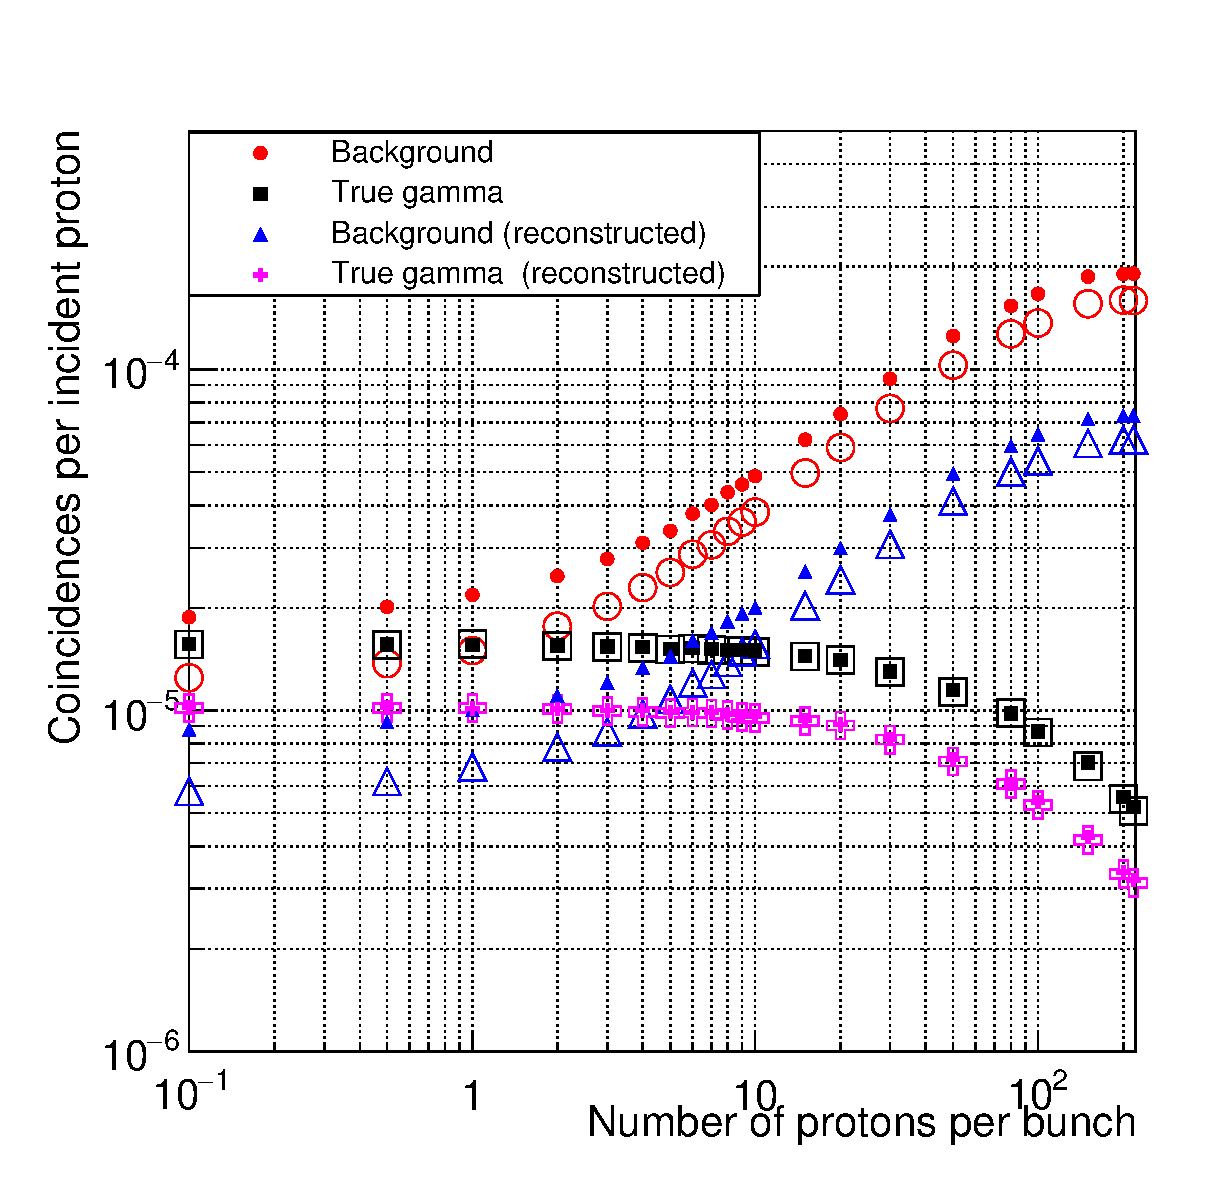
\includegraphics[width=0.5\textwidth]{./Figure/2017_06_28_Taux_coincidences_variation_protons_New_design_4EntreesLegend_LogXLogY.eps}}
 \subfloat[]{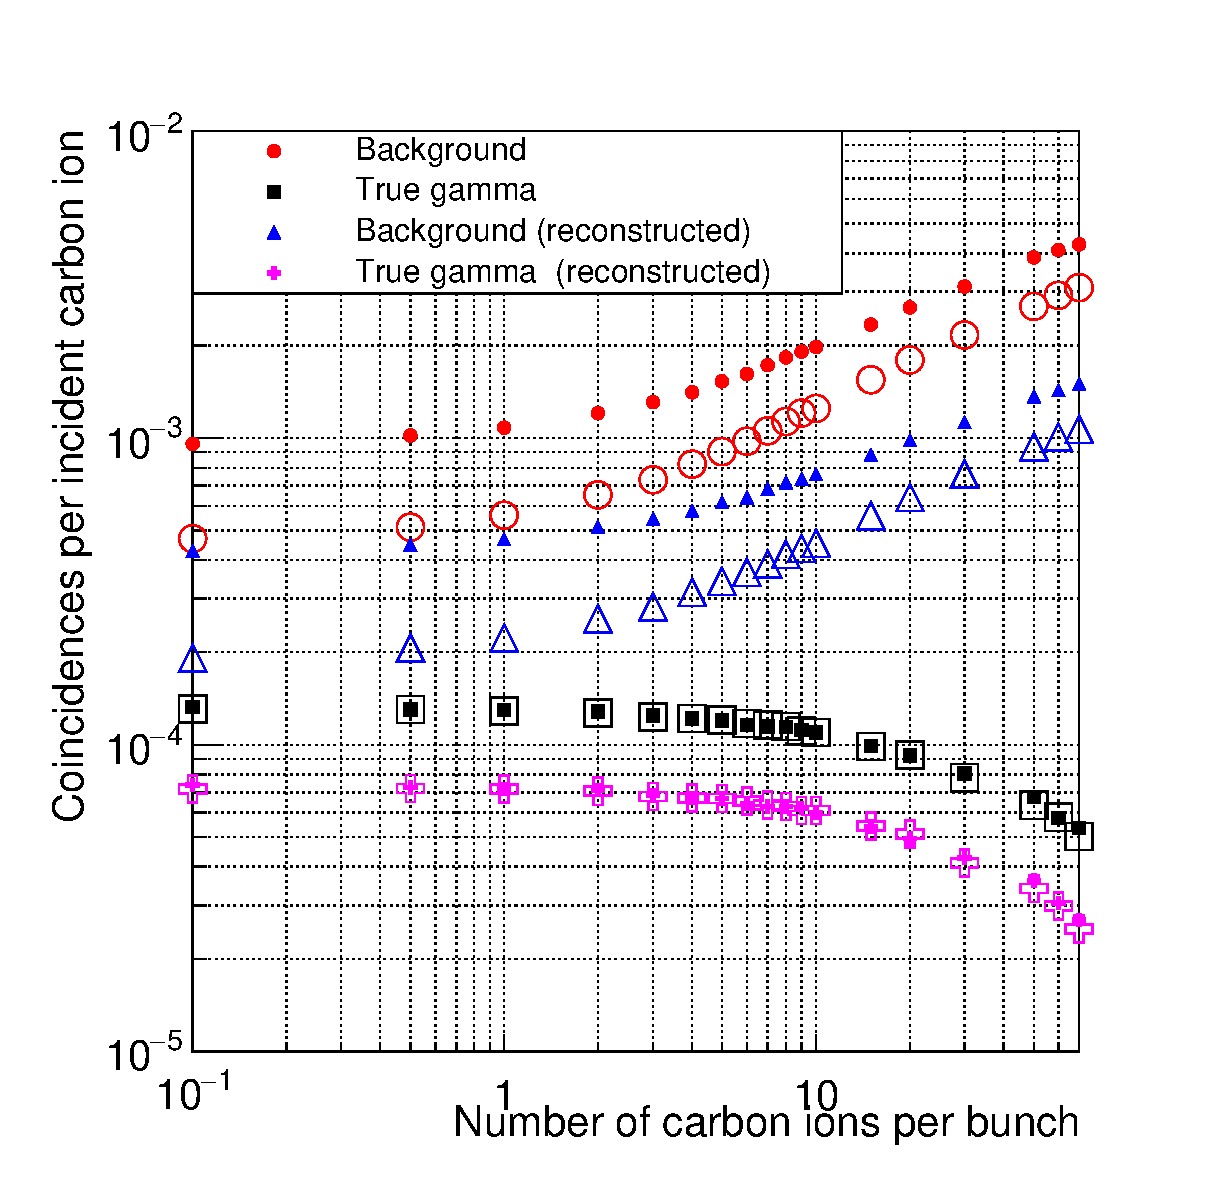
\includegraphics[width=0.5\textwidth]{./Figure/2017_06_28_Taux_coincidences_variation_carbonIons_New_design_4EntreesLegend_LogXLogY.eps}}
  \label{fig:coincidences}
\end{figure}

\newpage
At the clinical beam intensity, the high background level is mainly due to the random coincidences. In fact, the probability to detect two radiation coming from two different incident particles increases with the number of incident particles per bunch. Another issue is the single rate of events detected by each detector at those high intensities. For instance, at the clinic beam intensity in proton therapy, the single rate on the absorber is around 300 MHz and on the first silicon layer it is around 20 MHz. The current electronic front end and acquisition system are not able to treat this amount of data coming from all the detectors. As a result, it appears that it is impossible to use the Compton camera at a clinical beam intensity for the treatment monitoring in ion therapy.\newline
Nevertheless, if the intensity decreases enough to avoid almost all the random coincidences, the monitoring seems more feasible. In addition, it can be supposed that the time of flight discrimination will improve the signal to the background ratio at low intensities by suppressing the coincidences induced by charged particles. Indeed, the charged particles are slower than gamma rays which move at the light speed.

\subsection{Comparaison LM-MLEM vs Line cone reconstruction}


\begin{figure} [!h]
\subfloat[]{\includegraphics[width=0.5\textwidth]{./Figure/MLEM_2D.pdf}}
 \subfloat[]{\includegraphics[width=0.5\textwidth]{./Figure/MLEM_1D.pdf}}\\
  \subfloat[]{\includegraphics[width=0.5\textwidth]{./Figure/2015_02_16_Reconstruction_coinc_160MeVProton_TOF_6ns_file0to100_zoom.pdf}}
  \label{fig:comparaison}
\caption{LM-MLEM reconstruction for a proton beam at 160 MeV and $10^{8}$ incident protons. The events are detected in coincidence and the beam intensity is reduced to 1 proton per bunch. The PMMA target has a diameter of 15 cm and is 20 cm long. The Compton camera is centred at $y=+50 mm$. The time of flight discrimination is applied and 20 iterations are realized. The figure \ref{fig:fig_MLEM_CC_simulation_Hadronth_proton_reconstruction} represents the reconstruction in 2D for the plan (x,y). The position $x=0 mm$ is the center of the PMMA phantom and y axis the direction of the proton beam. The figure \ref{fig:fig_MLEM_CC_simulation_Hadronth_proton_profil} shows the profil corresponding to the figure \ref{fig:fig_MLEM_CC_simulation_Hadronth_proton_reconstruction} and following the axis y. The Bragg peak is localized at $y=+50 mm$. The figure \ref{fig:fig_LC_CC_simulation_Hadronth_proton_profil} is the profil obtained by means of line cone algorithm for the same simulation datas.}

\end{figure}

%   \begin{verbatim}
% a) 2015_10_20_Volume_100x100x5_voxels_and_size_20x40x1_source_Proton160MeV_camera_50mm_stat_2175events_sans_MatriceSensibility_bordYplusmoins-3_bordXplusmoins-3_median_iteration_10.
% b) 2015_10_20_Volume_100x100x5_voxels_and_size_20x40x1_source_Proton160MeV_camera_50mm_stat_2175events_sans_MatriceSensibility_bordYplusmoins-3_bordXplusmoins-3_selectionX_20mm_Filtre_median_iteration_Profil_Y_iteration_10. 
% c)  2015_02_16_Reconstruction_coinc_160MeVProton_TOF_6ns_file0to100_zoom               
%  \end{verbatim}

\subsection{Compton camera precision}


The information given by a control device as the Compton camera has to be viable and as precise as possible. In order to estimate the precision of the Compton camera, a method is used. 

\begin{figure}[!hbtp]	
\centering
\caption{The Compton camera precision is estimated with two different algorithms: line cone and LM-MLEM. The precision is given for $1\times10^{8}$ to $5\times10^{9}$ incident protons. A linear fit is realized in order to obtain the slope of the results (p1 parameter). The graphic is scaled in log-log. }	
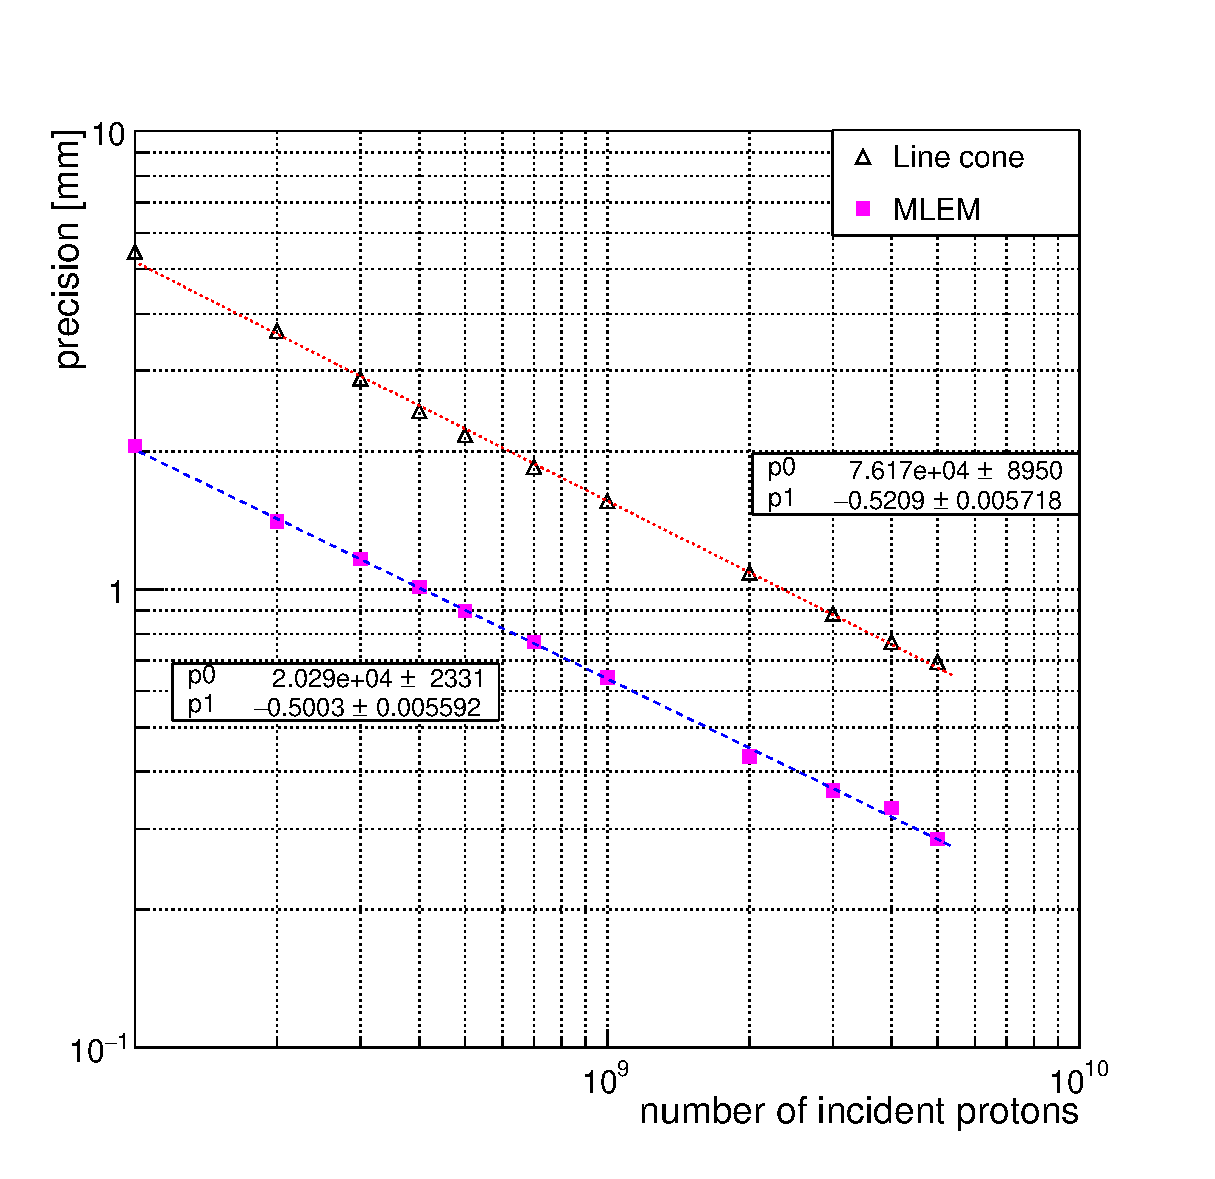
\includegraphics[width=0.7\textwidth]{./Figure/2017-10-21_Precision_Comparaison_linecone_MLEM_Article_Fit.eps}
\end{figure}



